% !Mode:: "TeX:UTF-8"

\chapter{动态温度管理技术基础}




因为我们持续减小芯片大小和要求高功耗下的性能,增长的芯片复杂性和功耗密度提高了芯片的峰值温度,也使温度梯度更加不均衡。
上升的峰值温度缩短芯片寿命,降低芯片性能,影响可靠性也增加散热成本\cite{skadron:TACO'04}。上升的温度和静态功耗之间有正反馈的关系,有可能造成热失控。
在多核或者众核系统中,不同的应用负载或许引起核之间功耗和温度的不平衡。温度在时间和空间上的变化产生的芯片局部温度最大值叫做高温点\cite{Donald:ISCA'06}。
过多的空间上的温度差也就是热梯度增加时钟抖动降低性能和可靠性。
上升的温度需要更多的散热能力去冷却处理器,一个典型的散热风扇会消耗高达服务器 $51\%$的功耗\cite{lefurgy2003energy}\cite{ayoub2010gentlecool}。


\section{温度不受管理的影响}\label{sec:adverse}

\subsection{温度对系统可靠性的影响}\label{sec:reliability}
高功耗的一个最明显的结果就是上升的芯片温度,高温对芯片最严重的的后果就是损害芯片的可靠性。
下面是温度相关的半导体器件失效机理\cite{jedec2003failure}:
%\begin{itemize}
%\item 电迁移(EM):(查的失效机理)由于传导电子和扩散金属原子之间的动量交换,金属线中例子会逐步移动,这样会导致金属线形变。甚至会引起金属线断开导致器件失效。
%\item 应力迁移(SM):金属原子在机械应力梯度下会发生移动导致金属线变形。不同材料的热膨胀率不同会产生应力。这个也会引起金属线断开导致器件失效。
%\item 介质击穿(DB):当介质中形成一个导电通路,电路的阴阳极短路时,介质失效。
%\end{itemize}
\begin{description}
\item[电迁移($EM$) :] ~由于传导电子和扩散金属原子之间的动量交换,金属线中离子会逐步移动,这样会导致金属线形变。它甚至会引起金属线断开导致器件失效。
\item[应力迁移($SM$) :] ~金属原子在机械应力梯度下会发生移动导致金属线变形。不同材料的热膨胀率不同会产生应力。这个也会引起金属线断开导致器件失效。
\item[介质击穿($DB$) :] ~当介质中形成一个导电通路,电路的阴阳极短路时,介质失效。
\end{description}

这些机理引起的失效时间($TF$)可以被表示为下式:
\begin{equation}
TF = A \cdot e^{E_a/(k \cdot T)}
\end{equation}
其中$A$ 是一个常数,$E_a$ 活化能量(eV),$k$ 是玻尔兹曼常数($8.62 \times 10^{-5}$ eV/K)。
这些都是正常数, $T$ 是器件的操作温度(K)。
所以, $TF$ 是温度的递减函数。
当温度上升时, $TF$ 会指数下降。这就意味着器件将极快速失效。

温度高不是系统可靠性问题的唯一原因。另外还有两个热现象即热循环和热梯度也会严重影响器件的可靠性。
热循环是操作温度的暂时波动,可能是由器件的正常功率上升或者下降引起。
另外也可能因为任务负载的变化或者设备的功耗管理策略,比如设备的部件在几种功耗模式下很频繁的切换。
热循环可以会削弱材料,引起介质裂开或者焊料疲劳等的不同失效。
热循环的失效率可以表示为:
\begin{equation}
\lambda \propto \Delta T^q
\end{equation}
其中$\Delta T$ 是热循环的幅度,$q$是热循环的频率。
温度波动越大或者越频繁,器件失效率就越大。

热梯度是整个芯片温度在空间上的不平衡。
因为现在片上系统(SoC)和多核众核芯片上负载不均衡,这样温度就会不平衡,引起大的温度梯度。
大的温度梯度最主要的影响是互连电阻不均衡,这会导致时钟偏差。这个是同步数字电路中很不希望发生的,会引起时序冲突。

\subsection{温度对静态功耗的影响}\label{sec:leakage}

温度不仅是功耗的结果,在某种程度上功耗和温度互为因果。
这是因为,静态功耗很大程度上取决于操作温度。当前静态功耗已经是系统总功耗的很明显的一部分,而且会随技术继续增长。
温度和静态功耗之间的关系已经被广泛的研究过\cite{liao2005temperature},漏电流可以表示为:
\begin{equation}
I_{leak} = I_s \cdot A \cdot T^2e^{\frac{\alpha + \beta V_{dd}}{T}}+B
\end{equation}
其中, 对于指定的技术, $A$ 、 $B$ 、  $\alpha$ 、 $\beta$ 是温度无关的正常数。
$V_{dd}$ 是供电电压,$I_s$ 是在指定温度和供电电压下的基准漏电流。
我们可以看出温度对漏电流的影响是 $T^2e^{1/T}$ 。图~\ref{fig:leakage}是漏电流对温度的曲线。
\begin{figure}
  \centering
    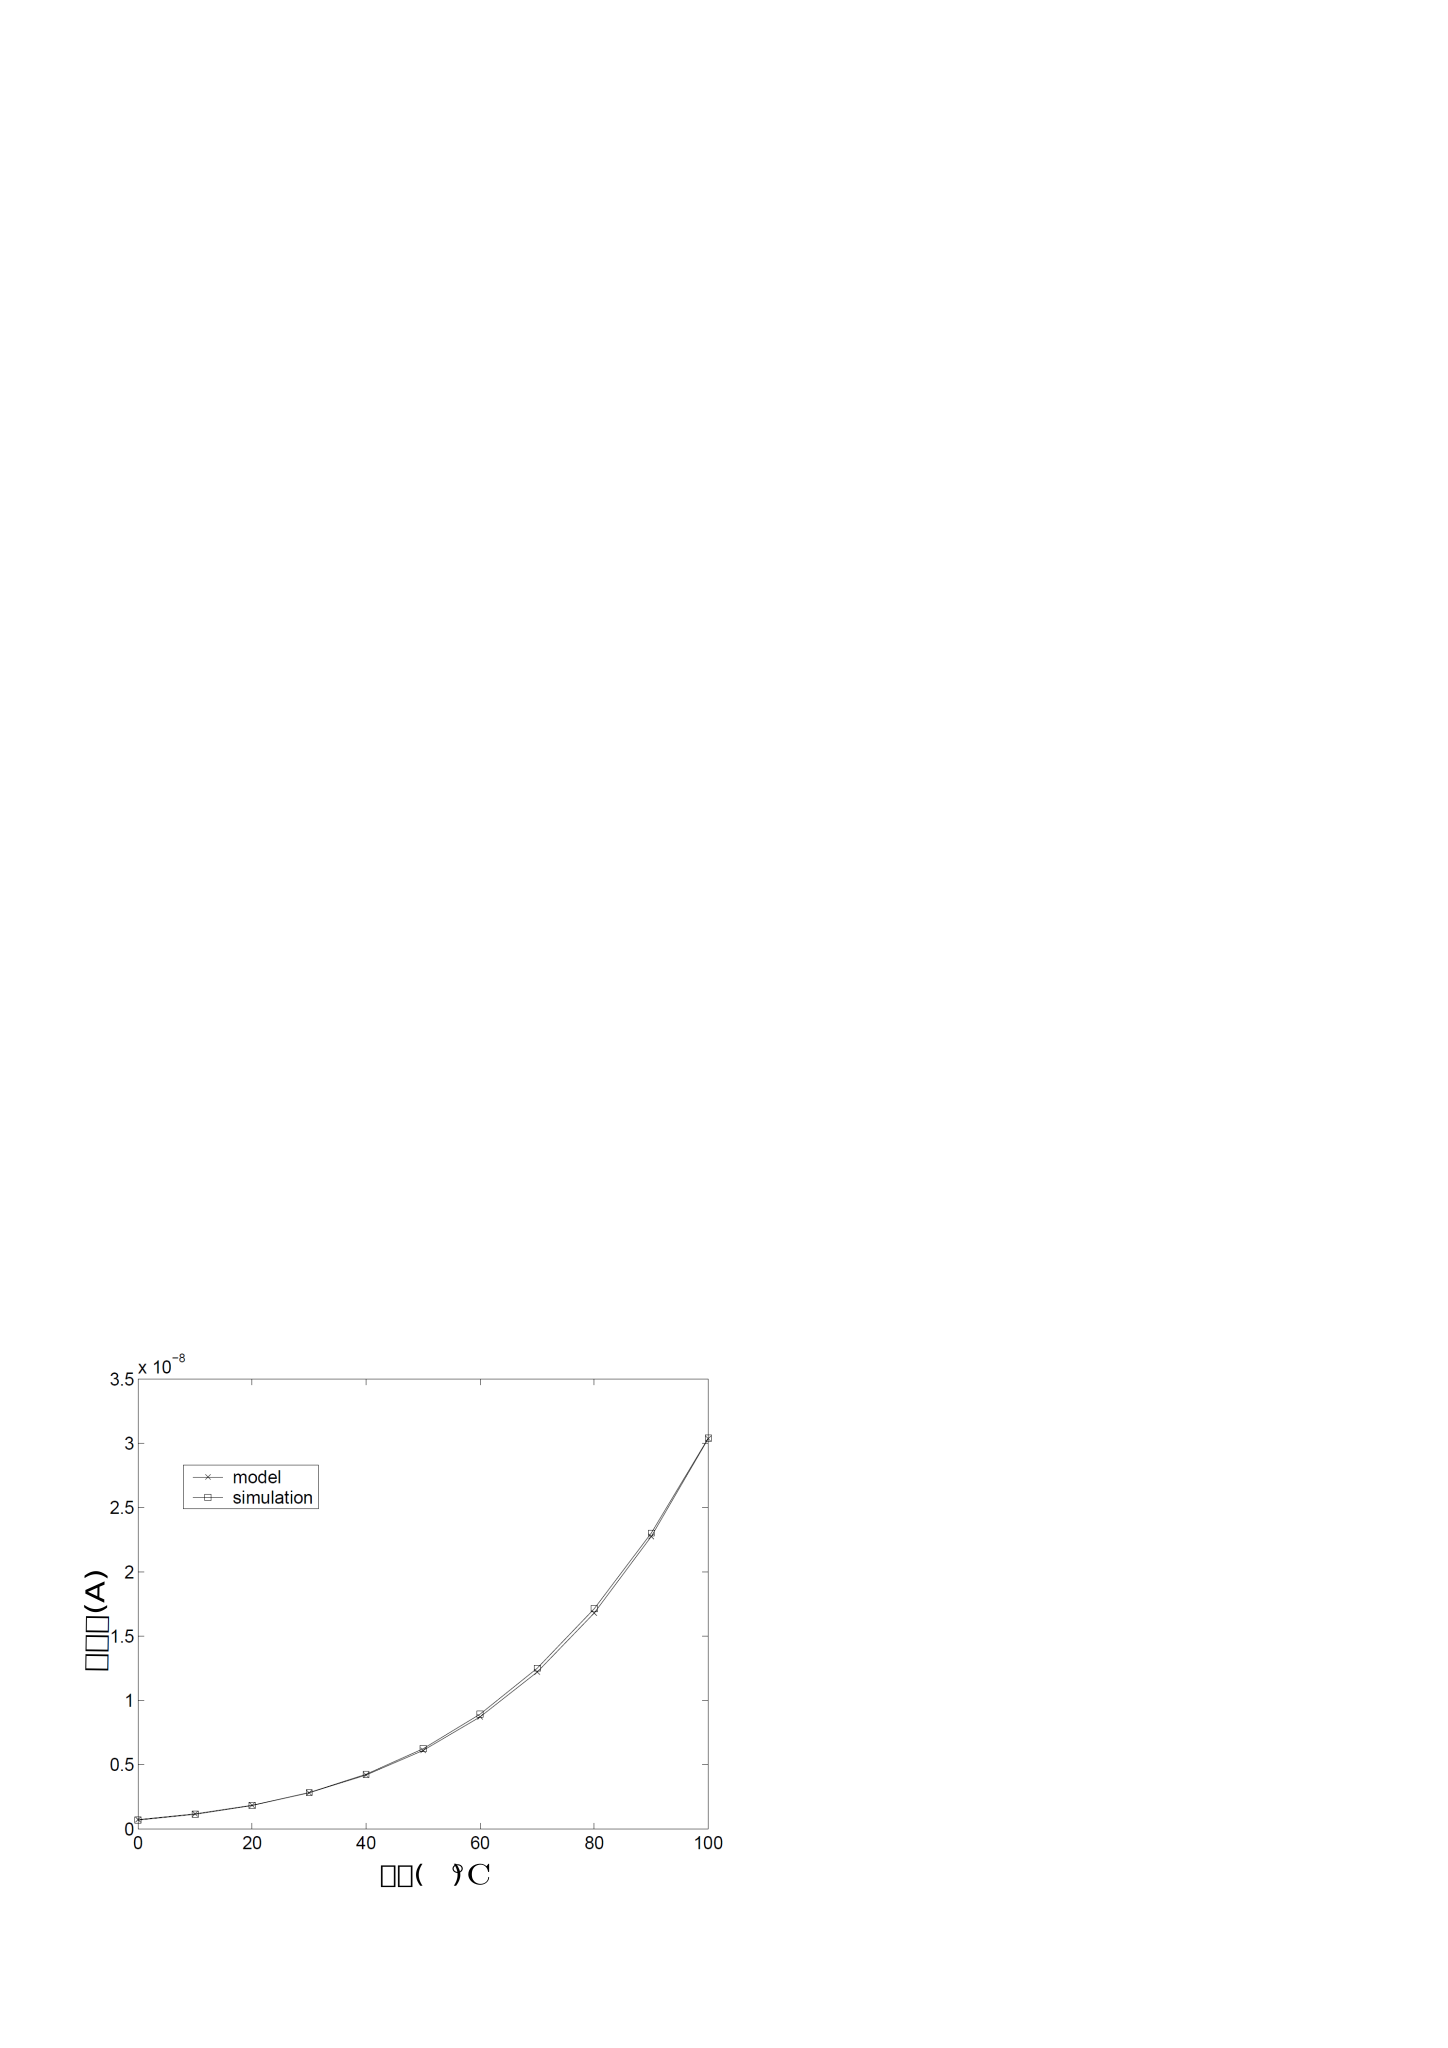
\includegraphics[width=0.7\columnwidth]{fig/leakage}
  \caption{温度与漏电流的关系\cite{zhang2003hotleakage}}\label{fig:leakage}
\end{figure}

\subsection{温度对冷却系统的影响}\label{sec:cooling}

上升的温度另一个明显的坏处就是冷却成本变得更高。
为了保证芯片正常运行,芯片不得不配备成本更高的封装来散热。
对于常规散热风扇型的冷却方法,散热风扇不得不在一个更高的速度上运行来散去芯片产生的额外的热量。
这是因为散热器的散热能力是由热阻$R_{h2a}$ (R2a表示从散热器到外部环境)决定,热阻$R_{h2a}$又是由散热风扇速度决定的,如下式:
\begin{equation}\label{eq:cooling}
R_{h2a} = (h_1v_f(1-e^{\frac{h_2v_f^{h_3}+h_4}{h_1v_f}}))^{-1}
\end{equation}

在式\eqref{eq:cooling}中,$h_1$ 、 $h_2$ 、 $h_3$ 、 $h_4$是芯片的特定物理系数,$v_f$ 是散热风扇速度。
风扇功耗 $P_{fan}$正比于风扇转速的立方,即 $P_{fan} \propto v_f^3$。
这意味着高的温度不仅是风扇功耗上升,同时也降低了风扇的使用寿命。

\section{动态温度管理技术}\label{sec:DTM}

前面已经说明,温度不受管理将会带来严重的可靠性,性能,功耗和成本的问题。
动态温度管理(DTM)技术就是用来解决上述问题,来控制芯片温度和功耗。
随着温度被调整,系统的可靠性就可以提升。适当的降低电子设备的温度 $10^{\circ}$C $\sim 15^{\circ}$C可以使设备寿命延长两倍。
对于金属结构,热循环幅度减少 $10^{\circ}$C 可以使平均失效时间增长16倍。
温度降低时静态功耗也会显著减少~\cite{kursun2006investigating}。温度每降低 $9^{\circ}$C ,静态功耗降低 50\%~\cite{liu2007accurate} 。
这对于将来的片上系统设计非常重要。因为静态功耗估计将会超过总功耗的 50\% 。
调控温度不仅能保证芯片可靠性和降低静态功耗,而且还能提升性能。在低温时,晶体管的开关速度更快~\cite{pamula2003cooling} 。
平衡的空间热梯度可以显著减轻时钟偏移问题。

动态温度管理需要能使芯片自主修改任务的执行和功耗特性的技术,以使低开销的冷却方法也能保证芯片在安全温度以内。
动态温度管理控制器在系统运行时监控系统信息,并采取相应的热管理措施。以最小的性能损耗,尽可能地把系统温度保持在安全阈值以下,尽尽量平滑地修正热分布。

对一个计算系统执行动态热管理,需要的最重要的系统信息是芯片温度。这个信息可以从片上温度传感器的到,或者用热模型估计。
一些最先进的动态温度管理技术还需要温度信息,应用程序特性,任务功耗等等。

\subsection{动态温度管理和动态功耗管理的不同}\label{sec:DPM}

尽管温度基本上是由功耗引起的,动态温度管理也需要修正功耗特性,甚至动态功耗管理和动态温度管理都用相同的措施想动态电压频率调整(DVFS)和任务迁移,
但是在动态功耗管理和动态温度管理上有几个明显的不同点。
首先,系统温度分布不仅仅只跟功耗分布相关。因为功耗可以瞬间改变,但是温度是功耗的的积累,在时间和空间上改变都很慢。
打个比方,功耗就像 RC 电路中的电流源,温度就像各个节点的电压。
所以温度的行为就像一个低通滤波器,滤掉了功耗变化中的高频部分。
第二,温度正比于功耗密度 , $ T \propto T/A$,这里 $A$ 是面积。
所以即使不能降低功耗,我们可以分配功耗到更大的面积上,这样仍然可以降低温度。
比如所有进程都合并在一个核上,芯片上这一小部分的负载很重,最好从散热的角度将他们分配到多个核上。
第三,比起温度管理策略,功耗管理策略可能有冲突的目标,有产生不期望的温度分布的可能。
比如,功耗管理策略可能为了节省功耗非常频繁的将器件切换到低功耗状态。
\ref{sec:reliability}节中提到过这个调整会产生大幅度和频繁的热循环,加速封装疲劳。
为了实现低功耗,功耗管理策略可能关掉一些部件整合计算,这会产生局部高温点和大的温度梯度。





















%我们已经进入众核处理器时代\cite{MaWang:APCCAS'14}.
%2012年,英特尔正式将第一代集成众核产品,代号为Knights Corner的协处理器推向市场。
%这一代产品使用P54C核心构建,片上集成61个CPU核心,实现了GPU级别的浮点运算速度。
%英特尔至强披™协处理器X100系列(代号为“Knights Corner”)是第一代英特尔®集成众核(英特尔®MIC)架构,
%它结合了许多英特尔的CPU内核在单一芯片上的。
%该生产线是针对高度并行的工作负载在各种领域,如计算物理,化学,生物和金融服务。
%Knights Corner片上集成了高达61核心。